\documentclass[letterpaper]{article}
\usepackage{aaai}
\usepackage{times}
\usepackage{helvet}
\usepackage{courier}
%\usepackage{cite}
\usepackage{url}
\usepackage{graphicx}
\usepackage{subfigure}
\usepackage{color}
\usepackage{tablefootnote}
\usepackage{footnote}
\usepackage{multirow}
\newcommand{\red}[1]{\textcolor{red}{#1}}

\frenchspacing
\setlength{\pdfpagewidth}{8.5in}
\setlength{\pdfpageheight}{11in}
%\setlength\titlebox{2.5in}
%\pdfinfo{
%/Title (Do You Want The Good or The Bad News First?: \\Analyzing Online News Headlines Polarity )
%/Author (Julio Cesar S. Reis, Fabricio Benevenuto)}
\setcounter{secnumdepth}{0}
 \begin{document}
% The file aaai.sty is the style file for AAAI Press
% proceedings, working notes, and technical reports.
%
%\title{Do You Want The Good or The Bad News First?: \\Analyzing Sentiments of Online News Headlines}
%\title{The Breaking News Effect: Characterizing Online News Headlines}
\title{The H-index Paradox: Your Coauthors Have Higher H-index than You}

%\author{J\'ulio Reis\\ UFMG, Brazil\\ \url{julio.reis@dcc.ufmg.br}
%\And Fabr\'icio Benevenuto\\ UFMG, Brazil\\ \url{fabricio@dcc.ufmg.br}
%}

%\author{Julio Cesar S. Reis\\
%Federal University of Minas Gerais, Brazil\\
%\textit{julio.reis@dcc.ufmg.br}\\
%2275 East Bayshore Road, Suite 160\\
%Palo Alto, California 94303\\
%}

\maketitle
\begin{abstract}
\begin{quote}

One interesting phenomena that emerges from the typical structure of social networks is the Friendship Paradox. It states that your friends have on average more friends than you do. Recent efforts have explored variations of it, with numerous implications for dynamics in social networks.
However, the friendship paradox and its variations have considered only the topological structure of networks, neglecting many other personal characteristics that are correlated with node degree. In this paper we take the case of scientific collaboration to investigate if a similar paradox also arises in terms of individuals scientific productivity measured through their h-index. H-index is a metric widely used in academia to capture both quality and quantity of an individual's scientific output. It is natural to expect that a researcher may use her coauthors' h-indexes as a way to infer whether her own h-index is adequate in her research area. Nevertheless, in this paper, we show that the average h-index of a researcher's coauthors is usually greater than her own h-index. We present empirical evidence of this paradox and discuss some of its potential consequences.
\end{quote}
\end{abstract}

\section{Introduction}

One interesting phenomena that emerges from the typical structure of social networks is the Friendship Paradox. It states that your friends have on average more friends than you do. It basically exists because of the heterogeneity of degrees in typical social networks. Individuals with high number of friends are over represented when averaging over friends \cite{quatro}. This paradox and variations of it have important implications for the evolution of networks and for applications that explore dynamic aspects of social networks like information spreading. For example,
a recent effort verified two new paradoxes: the \textit{virality paradox} that states that your friends receive more viral content than you and the \textit{activity paradox} that states that your friends are more active than you. This last one is important to help regulating information overwhelming \cite{tres}. A recent effort attempts to generalize the friendship paradox to complex networks by exploring the paradox in collaboration networks \cite{eom2014generalized}. Based on the identified paradox, the authors propose effective sampling for identifying high characteristic nodes in large scale networks.

These important recent efforts verified the existence of the friendship paradox considering only the topological structure of social networks. However, the paradox may also arise in many other personal characteristics that are correlated with node degree, which has not yet been well examined. In this paper we take the case of scientific collaboration to investigate if the paradox also arises in terms of individuals' scientific productivity measured through their h-index.

%Particularly, As the structure is directly associated productivity, we want to know if the paradox also reaches metrics to measure prolificness. We are particularly interested in the
H-index~\cite{Hirsch:2005} is a metric originally proposed to measure an individual's scientific output \cite{dois}. Its calculation is quite simple as it is based on the researcher's set of most cited publications and the number of citations they have received.  More specifically, a researcher has an h-index $h$ if she has at least $h$ publications that have received at least $h$ citations. Thus, if a researcher has 10 papers with at least 10 citations, her h-index is 10.

Like any metric that attempts to summarize in a single number a complex and subjective evaluation, h-index has its limitations, including being biased towards the researcher’s scientific lifetime, not accounting for the number of coauthors in the publications and ignoring the distinct citation patterns across different areas. Nevertheless, the h-index became popular as it provides a notion of both quality and quantity of a researcher's scientific output in a simple and easy to compute metric.

Often, researchers are tempted to evaluate themselves based on h-index. Systems like Google Scholar\footnote{\url{http://scholar.google.com/intl/en/scholar/citations.html}}  and ArnetMiner\footnote{\url{http://arnetminer.org}} help researchers track their publication impact and coauthors, as well as to maintain their profiles, where the h-index is clearly stamped. Thus, it is natural to assume that researchers may use their coauthors' h-indexes as a way to estimate whether they, themselves, have an adequate h-index in their respective research areas or within a department or university.
%For instance, if you search Google Scholar for a piece of your email %(e.g., dcc.ufmg.br) you can obtain a ranking of your department colleagues according to their citation numbers.
This paper seeks to show that this kind of comparison may lead to the \textit{h-index paradox}. In other words, we show that the average h-index of a researcher's coauthors is usually greater than her own h-index. We further explore potential consequences of this paradox to academics.

Next, we briefly discuss how we have estimated the h-index for researchers from distinct computer science research communities, and then we provide empirical results on the measurement of the h-index of those researchers and their coauthors.


\section{Estimating H-index}


In order to provide evidence of the h-index paradox, we need to be able to (1) identify the coauthors of a large set of researchers and (2) estimate the h-index of these researchers as well as of their respective coauthors.

We focus on constructing the coauthorship network of Computer Science researchers of different areas. To do that we gathered data from DBLP\footnote{\url{http://www.informatik.uni-trier.de/~ley/db/}}, as it offers its entire database in XML format for download. We gathered this data for those researchers who published in the flagship conferences of 10 major ACM SIGs (Special Interest Groups): SIGDOC, SIGCHI, SIGIR, KDD, SIGCOMM, SIGGRAPH, SIGMETRICS, POPL, and SIGMOD.

There are several tools that measure the h-index of researchers, out of which Google Scholar is today the most prominent one. However, to have a profile in this system, a researcher needs to sign up and explicitly create it. In a preliminary collection of part of the profiles of the DBLP authors, we found that less than 30\% of these authors had a profile at Google Scholar%~\cite{um}
~(citation omitted due to the double blind process). Thus, this strategy would largely reduce our dataset.

To overcome this limitation, we used data from the SHINE (Simple HINdex Estimator) project\footnote{\url{http://shine.icomp.ufam.edu.br}} to estimate the researchers' h-index. SHINE provides a website that shows the h-index of almost two thousand Computer Science conferences. It was created based on a large scale crawl of Google Scholar. Its strategy consisted of searching for the title of all papers published in several conferences, thus effectively estimating conferences’ h-index based on the citations computed by Google Scholar. Although SHINE only allows one to search for the h-index of conferences, the SHINE developers kindly allowed us access to their dataset to infer the h-index of researchers based on the conferences they crawled.


\begin{figure}[!htb]
\centering
 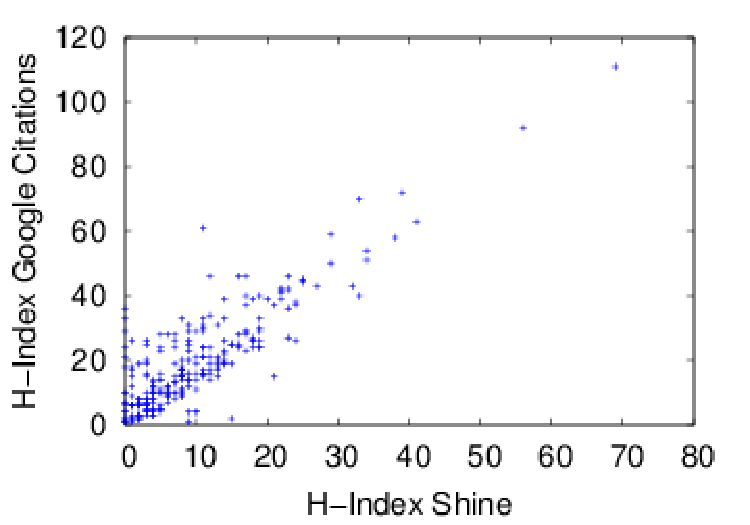
\includegraphics[width=.46\textwidth]{figures/hindex_scatter_plot.pdf}
\caption{Correlation between the inferred h-index and Google Citations one}
\label{fig:hindex_scatter_plot}
\end{figure}

As SHINE only covers conferences and even though does not track all existing conferences in Computer Science, researchers' h-index might be underestimated when computed with this data. To investigate this issue, we compared the h-index of a set of researchers with a profile on Google Scholar with their estimated h-index based on the SHINE data. For this, we randomly selected 10 researchers for each of the ACM SIG's flagship conferences and extracted their h-indexes from their Google Scholar profiles. In comparison with the h-index we estimated from SHINE, the Google Scholar values are, on average, 50\% higher. 
Figure~\ref{fig:hindex_scatter_plot} shows the scatter plot for the two h-index measures. We can note that although SHINE h-index is smaller, the two measures are highly correlated. The Pearson's correlation coefficient is 0.85, which indicates that researchers have proportional h-index estimations in both systems.



\begin{table*}[t]
\centering
\caption{The DBLP data of the 10 ACM SIG flagship conferences.}
\label{tab:sigs_conference_period}
{\small
\begin{tabular}{|l|l|c|c|c|c|c|c|c|c|} \hline
SIG & Conference & Period & H-Index & Authors & Publications & Editions & Aut/Edi & Pub/Edi & Aut/Pub\\ \hline
SIGCHI & CHI & 1994-2012 & 144 & 5095 & 2819 & 19 & 268.16 & 148.37 & 1.81\\ \hline
SIGCOMM & SIGCOMM & 1988-2011 & 140 & 1593 & 796 & 24 & 66.38 & 33.17 & 2.00\\ \hline
SIGDOC & SIGDOC & 1989-2010 & 23 & 1071 & 810 & 22 & 48.68 & 36.82 & 1.32\\ \hline
SIGGRAPH & SIGGRAPH & 1985-2003 & 119 & 1920 & 1108 & 19 & 101.05 & 58.32 & 1.73\\ \hline
SIGIR & SIGIR & 1978-2011 & 116 & 3624 & 2687 & 34 & 106.59 & 79.03 & 1.35\\ \hline
SIGKDD & KDD & 1995-2011 & 124 & 3078 & 1699 & 17 & 181.06 & 99.94 & 1.81\\ \hline
SIGMETRICS & SIGMETRICS & 1981-2011 & 71 & 2083 & 1174 & 31 & 67.19 & 37.87 & 1.77\\ \hline
SIGMOD & SIGMOD & 1975-2012 & 147 & 4202 & 2669 & 38 & 110.58 & 70.24 & 1.57\\ \hline
SIGPLAN & POPL & 1975-2012 & 85 & 1527 & 1217 & 38 & 40.18 & 32.03 & 1.25\\ \hline
SIGCSE & SIGCSE & 1986-2012 & 51 & 3923 & 2801 & 27 & 145.30 & 103.74 & 1.40\\ \hline
\end{tabular}
}
\end{table*}


Table~\ref{tab:sigs_conference_period} summarizes this data, including the SIG, the conference acronym, the period
considered (some conferences had the period reduced to avoid hiatus in the data), the h-index and the total number of authors, publications and editions as well as ratios extracted from these last three figures. This dataset is useful to our propose as it allows us to investigate the h-index paradox on real Computer Science communities, in which researchers might tend to compare themselves with other peers.


\section{Comparing the H-index of a Researcher with her Coauthors'}



Having accurately estimated the h-index of each researcher, we can compare it with her coauthors'. Figure~\ref{fig:comp} shows the fraction of authors with h-index smaller than the average of their coauthors for the 10 conferences we have considered. We note that even focusing on authors that have published in flagship conferences of ACM SIGs, the fraction of authors that are below the average is quite high for all research communities analyzed, varying from 69\% to 81\%. When we look at the percentage of authors with at least one coauthor with higher h-index than hers, the numbers are higher than 90\% for most of the conferences.


\begin{figure*}[t]
  \centering
  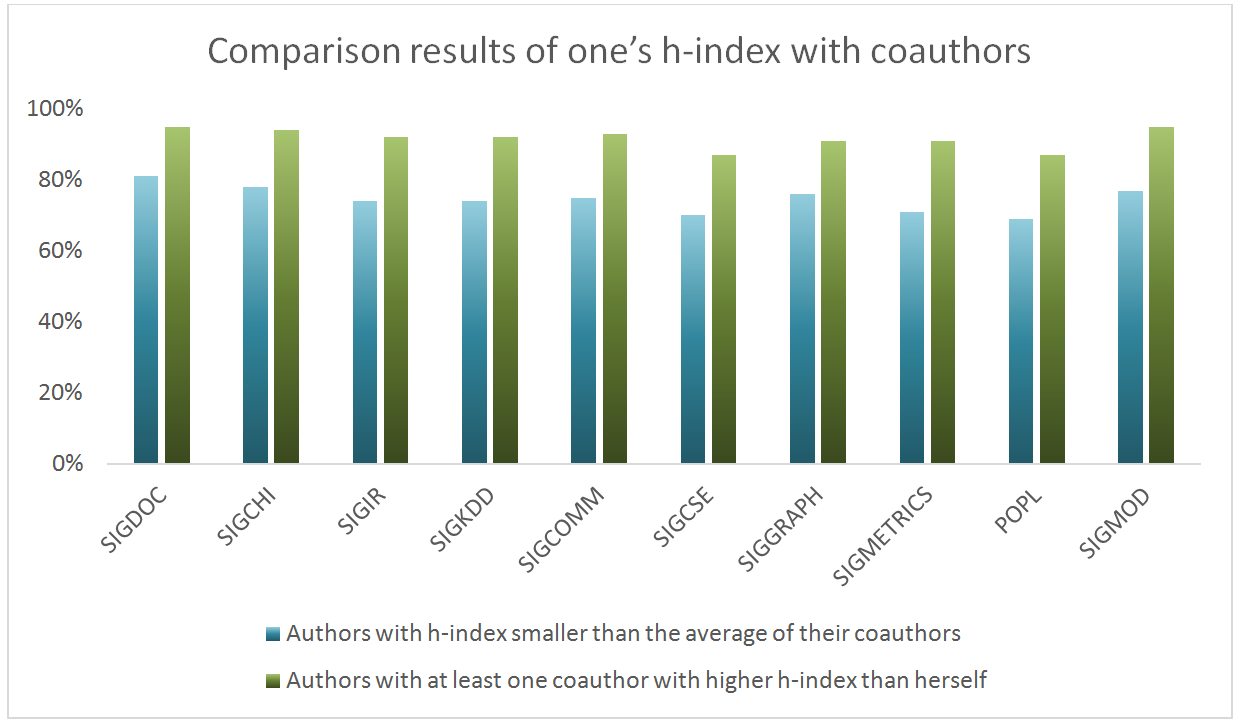
\includegraphics[width=.77\textwidth]{figures/fig1.png}
  \caption{Comparison results of one's h-index with her coauthors'}
  \label{fig:comp}
\end{figure*}


These results confirm the h-index paradox since one's coauthors in a research community have, on average, a higher h-index than her. The reasons behind the h-index paradox might be explained by the high correlation between degree and h-index in a research community. Usually, high degree nodes tend to be senior researchers that not only form a large number of students but also establish more collaborations and with different groups along their career. To further investigate this issue, Figure~\ref{fig:distrib} shows the distribution of the number of authors as a function of h-index. It clearly resembles a long tail distribution, suggesting that some authors disproportionally contribute to the average h-index. This disproportion on the average h-index might be even accentuated with the typical structural properties of coauthorship networks, which are similar to many social networks \cite{seis} \cite{oito} - i.e., they have a long tail degree distribution, where highly connected authors create bridges across multiple highly connected components, leading to the properties of high clustering coefficient and short diameter. The correlation between a researcher's h-index and her degree is 0.36, which, although not so high, is positive, suggesting that some researchers have high h-index and are also more connected in the network.





\section{Concluding Discussion}

In this paper we have analyzed a variation of the well known friendship paradox. By analyzing the average h-index of a researcher's coauthors for different research communities in Computer Science, we show that the h-index paradox arises since h-index is highly correlated with node degree. Based on this observation, it is expected that a wide range of variations of this paradox might hold for any characteristic showing a positive correlation with degree. Such characteristics might be individual aspects related to some specific context like the h-index in scientific collaborations or they may be purely topological like various node centrality metrics that are usually correlated with degree, such as Pagerank \cite{page1999pagerank}.


\begin{figure}[!htpb]
  \centering
  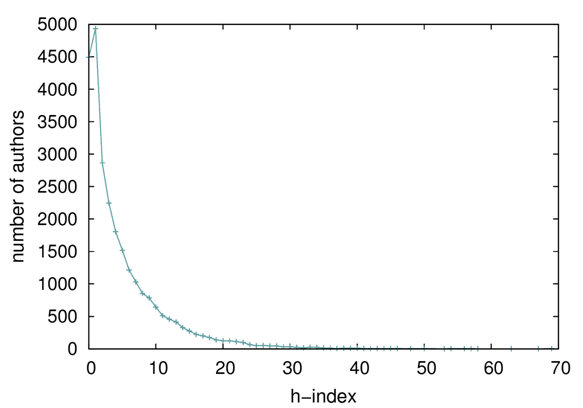
\includegraphics[width=.5\textwidth]{figures/fig2.png}
  \caption{Distribution of authors according to their h-indexes.}
  \label{fig:distrib}
\end{figure}


One of the implications of the friendship paradox is the fact that it leads to systematic biases in our perceptions. For example, there are studies that show that people think they drive better than their friends \cite{mckenna1991factors}. What the h-index paradox says to us is that researchers from different Computer Science communities might feel bellow the average in comparison with their coauthors, which is an instantiation of a sensation that occurs in different scenarios and is even culminated in an expression that is common to different languages and cultures: \textit{The neighbor’s grass is always greener on the other side.} While the process that governs citations is already quite complex \cite{barabasi1999emergence} \cite{onze}, we speculate that the sensation that comes from this paradox might also influence the behavior of some researcher, for example, motivating and pressuring her to reduce the sensation that she is below the average. Competition in science can be good as it gives extra motivation for researchers to work hard, but it also may lead to undesirable scenarios, especially when researchers cross ethical boundaries tempted to ``sell'' better their publications. One interesting direction for future work is to conduct a user study to confirm whether researchers tend to believe they have higher h-index than their colleagues or not, and also to attempt to identify whether this sensation motivates healthy competition or bad research practices.




%ACKNOWLEDGMENTS are optional
\section{Acknowledgments}
Omitted due to the double blind process. 
%This work was funded by grants from CNPq, CAPES and FAPEMIG.

%
% The following two commands are all you need in the
% initial runs of your .tex file to
% produce the bibliography for the citations in your paper.
\bibliographystyle{aaai}
%\small{\bibliography{references}} % sigproc.bib is the name of the Bibliography in this case
\bibliography{references} % sigproc.bib is the name of the Bibliography in this case

% You must have a proper ".bib" file
%  and remember to run:
% latex bibtex latex latex
% to resolve all references
%
% ACM needs 'a single self-contained file'!
%
%APPENDICES are optional
%\balancecolumns

\end{document}
